\chapter{Свободная энергия искажения ориентационной структуры}\label{ch:ch1}

В данной работе изучается изменение ориентационной структуры ХЖК, находящегося между двумя плоскопараллельными пластинами, расположенными на расстоянии  $L$ друг от друга. Ограничивающие пластины считаются проводящими, и к ним подведено постоянное напряжение $U$, таким образом, система имеет вид плоского конденсатора. При изменении напряжения $U$ может меняться ориентация директора в ячейке. Изучению таких трансформаций структуры будет уделено основное внимание.
\begin{figure}[ht]
	\centering
	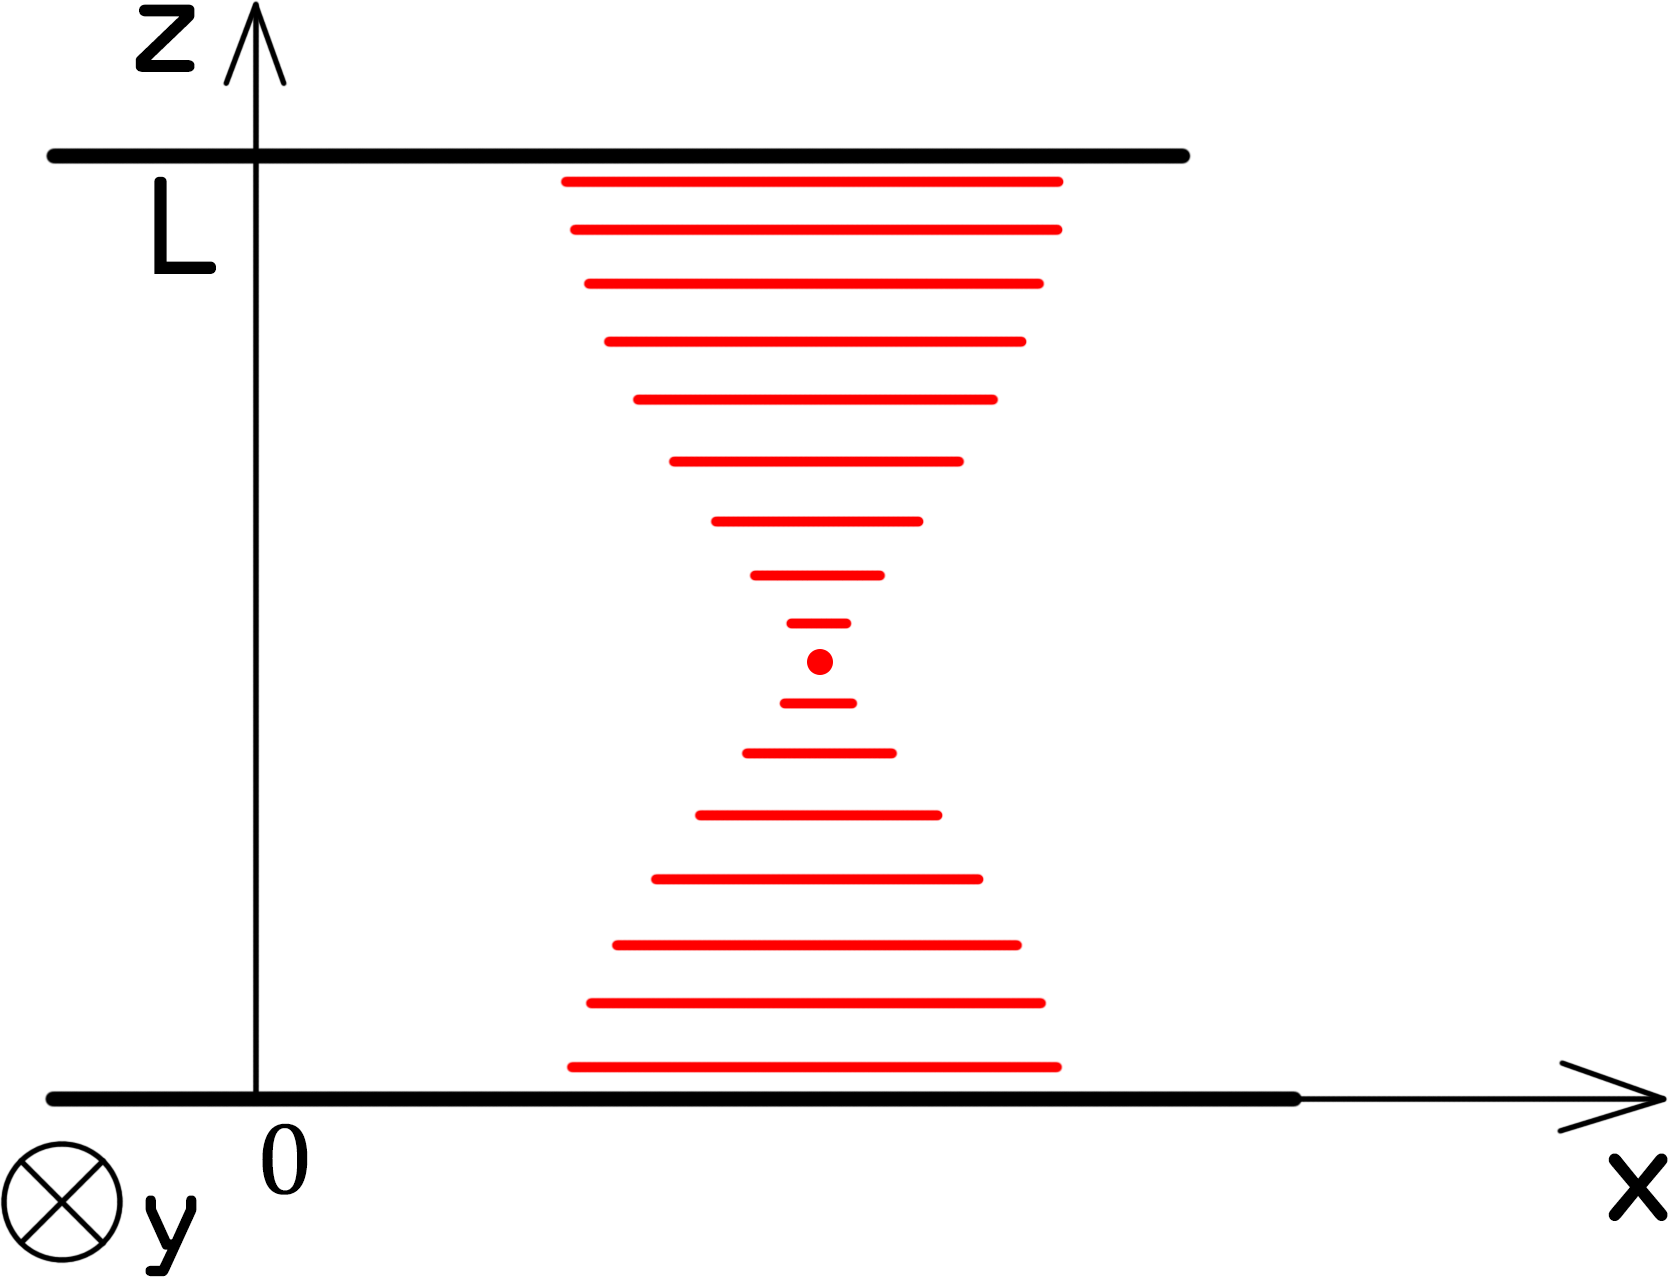
\includegraphics[width=10cm]{decart}
	\caption{Декартова система координат для ячейки ХЖК с планарной геликоидальной структурой.}
	\label{pic:decart}
\end{figure}

Введём декартову систему координат с осью $z$, направленной перпендикулярно пластинам (Рис.~\ref{pic:decart}).
Предположим, что размер ограничивающих пластин значительно превосходит расстояния $L$ между ними, таким образом, можно пренебречь краевыми эффектами.
Также предположим, что все физические характеристики рассматриваемой системы однородны в плоскости $XY$ и зависят только от координаты $z$: $\textbf{n}(\textbf{r}) = \textbf{n} (z)$, $\textbf{E} = \textbf{E}(z)$, где $\bb{E}$ - напряжённость электрического поля.

Свободная энергия ХЖК, связанная с искажением ориентационной структуры директора, может быть представлена в виде суммы четырёх слагаемых~\eqref{F_tot very basic}
\begin{equation}
\FF_\mathrm{tot} = \FF_\mathrm{e} + \FF_\mathrm{sf} + \FF_\mathrm{f} + \FF_\mathrm{flex}.
\label{F_tot very basic}
\end{equation}
Здесь $\FF_\mathrm{e}$ -- вклад в свободную энергию, связанный с ориентационной упругостью в объёме, $\FF_\mathrm{sf}$ -- упругая энергия сцепления молекул ЖК с ограничивающими поверхностями, $\FF_\mathrm{f}$ -- энергия ЖК как диэлектрика во внешнем электрическом поле, $\FF_\mathrm{flex}$ -- вклад в свободную энергию, обусловленный взаимодействием флексоэлектрической поляризации с внешним электрическим полем. Эти слагаемые можно естественным образом разделить на две группы: обусловленные ориентационной упругостью (первые два слагаемых в~\eqref{F_tot very basic}) и возникающие из-за взаимодействия ЖК с внешним полем (третье и четвёртое слагаемые в~\eqref{F_tot very basic}).

\section{Свободная энергия упругих искажений ориентационной структуры}\label{sec:ch1/sec1}
Первое слагаемое в~\eqref{F_tot very basic}, свободная энергия упругих ориентационных искажений $\FF_e$, было впервые описано в работах Озена~\autocite{Oseen1933} и Цохера~\cite{Zocher1933} и более подробно изучено Франком~\autocite{Frank1958}. Этот вклад может быть записан как~\cite{deGennesbook1995}
\begin{equation}
\FF_\mathrm{e} = \frac{S_\perp}{2} \int\limits_{l_1}^{l_2}\left[ K_{11} (\diver{\textbf{n}})^2 + K_{22} (\textbf{n}\rot{\textbf{n}} + q_0)^2 + K_{33} (\textbf{n}\times \rot{\textbf{n}})^2 \right]\, dz.
\label{F_e from n}
\end{equation}
Здесь $S_{\perp}$ -- площадь ограничивающих пластин, $K_{ii}$ -- модули Франка, $\pi/q_0$ -- период геликоидальной спирали ХЖК.
Физический смысл констант $K_{ii}$ удобно пояснить на примере свободной энергии Франка для нематического ЖК, которая получается из~\eqref{F_e from n} при $q_0 = 0$.
Тогда каждое из трёх слагаемых подынтегрального выражения соответствует искажениям определённого типа.
При деформации поперечного изгиба (Рисунок~\ref{distortions}a) в правой части~\eqref{F_e from n} остаётся только слагаемое с $K_{11}$.
При деформации кручения (Рисунок~\ref{distortions}b) в правой части~\eqref{F_e from n} остаётся только слагаемое с $K_{22}$.
Наконец, при деформации продольного изгиба (Рисунок~\ref{distortions}c) остаётся только слагаемое с $K_{33}$.
Таким образом, $K_{11}$, $K_{22}$ и $K_{33}$ являются модулями поперечного изгиба, кручения и продольного изгиба соответственно.

\begin{figure}
	\centering
	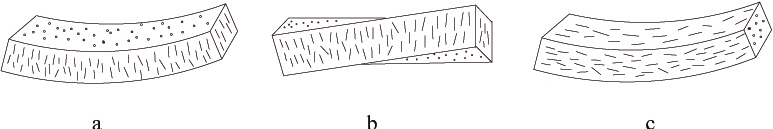
\includegraphics[width=15cm]{ThreeDistortions}
	\caption{Различные типы деформаций поля директора в ЖК: a -- поперечный изгиб, b -- кручение, c -- продольный изгиб.}
	\label{distortions}
\end{figure}

Для дальнейшего анализа свободной энергии удобно представить декартовы координаты директора $\bb{n}(z)$ как функции полярного угла $\theta(z)$ и азимутального угла $\varphi(z)$ (Рисунок~\ref{Coords}):
\begin{equation}
\bb{n} = 
\begin{pmatrix}
\sin{\theta}\cos{\phi}\\
\sin{\theta}\sin{\phi}\\
\cos{\theta}
\end{pmatrix}.
\end{equation}

\begin{figure}[ht]
	\centering
	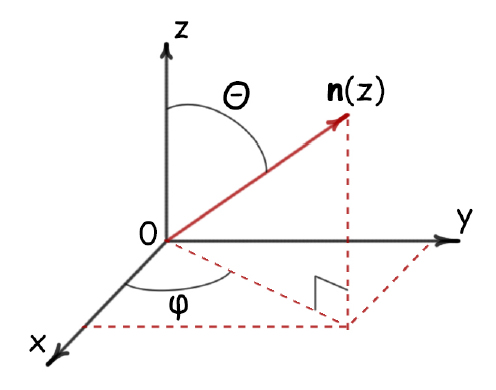
\includegraphics[width=7cm]{pic_04}
	\caption{Полярный $\theta(z)$ и азимутальный $\phi(z)$ углы директора $\bb{n}(z)$.}
	\label{Coords}
\end{figure}
Для $\diver{\bb{n}}$ и $\rot{\bb{n}}$ имеем:
\begin{equation}
\begin{split}
&\diver{\bb{n}} = -\theta' \sin{\theta},\\
&\rot{\bb{n}} = \begin{pmatrix}-\theta'\cos{\theta}\sin{\phi}-\phi'\sin{\theta}\cos{\phi}\\\theta'\cos{\theta}\cos{\phi}-\phi'\sin{\theta}\sin{\phi}\\0\end{pmatrix}.
\end{split}
\label{div and rot}
\end{equation}
Здесь штрихом обозначена производная по $z$. Подставляя~\eqref{div and rot} в~\eqref{F_e from n}, получаем
\begin{equation}
\FF_\mathrm{e} =\FF^\mathrm{(0)}_{e} + \frac{S_\perp}{2} \int\limits_{0}^{L}\left[ \AA(\theta) (\theta')^2 + \BB(\theta) (\phi ' )^2 - \CC(\theta)\phi' \right]\, dz.
\label{eq:F_e_basic}
\end{equation}
\begin{equation}
\begin{aligned}[c]
\AA (\theta) &= K_{11}\sin^2{\theta} + K_{33}\cos^2{\theta},\\
\BB (\theta) &= \sin^2{\theta} \left( K_{22}\sin^2{\theta} + K_{33}\cos^2{\theta}  \right),\\
\CC (\theta) &= q_0 K_{22}\sin^2{\theta}.
\end{aligned}
\end{equation}
где $\FF^\mathrm{(0)}_{e} = VK_{22}q_0^2/2$, а $V = S_\bot L$ -- это объём ячейки.

Второе слагаемое в выражении~\eqref{F_tot very basic} -- энергия сцепления ХЖК с подложкой:
\begin{equation}
\FF_\mathrm{sf} = \frac{S_\perp}{2}\sum\limits_{\alpha=1,2} w_\alpha \left( \textbf{n}(l_\alpha),\, \textbf{n}^{(\alpha)}_0 \right), \quad l_1 = 0, \quad l_2 = L.
\label{F_bound very basic}
\end{equation}
Здесь индекс $\alpha = 1,2$ нумерует границы, скалярные функции $w_\alpha$  зависят от направлений директора на границах ячейки $\textbf{n}(l_\alpha)$, а также от направления осей лёгкого ориентирования $\textbf{n}^{(\alpha)}_0$.
Важное свойство функций $w_\alpha$ в~\eqref{F_bound very basic} -- обращение соответствующей функции в ноль, если $\bb{n}(l_\alpha) = \bb{n}^{(\alpha)}_0$. Конкретный вид $w_\alpha$ выбирается в соответствии с решаемой задачей.
Так, в случае малых отклонений $\bb{n}(l_\alpha)$ от $\bb{n}^{(\alpha)}_0$ возможно использование квадратичной аппроксимации по разности этих векторов:
\begin{equation}
w_\alpha(\bb{n}(l_\alpha),\ \bb{n}^{(\alpha)}_0) = w_\alpha(\bb{n}(l_\alpha) - \bb{n}^{(\alpha)}_0) = (\bb{n}(l_\alpha) - \bb{n}^{(\alpha)}_0) \hat{W}_\alpha (\bb{n}(l_\alpha) - \bb{n}^{(\alpha)}_0)
\label{Square_approximation_matrices}
\end{equation}
Здесь $\hat{W}_\alpha$ -- положительно определённые матрицы размера $3\times 3$.
Потенциал~\eqref{Square_approximation_matrices} является квадратичным по отклонениям директора на границах. Также применяется потенциал, квадратичный по отклонениям углов и использованный, например, в~\cite{VAR2013}:
\begin{equation}
w_\alpha(\theta_\alpha,\phi_\alpha, \theta_0^{(\alpha)}, \phi_0^{(\alpha)}) = W^{(\alpha)}_\theta \left( \theta_\alpha - \theta^{(\alpha)}_0 \right)^2 + W^{(\alpha)}_\phi \left( \phi_\alpha - \phi^{(\alpha)}_0 \right)^2.
\label{Square_approximation}
\end{equation}
Здесь $W^{(\alpha)}_{\theta,\, \phi} > 0$ -- константы сцепления с подложкой, $\theta^{(\alpha)}_0$ и $\phi^{(\alpha)}_0$ -- углы лёгкого ориентирования на границах, также введены обозначения: $\theta_1 = \theta(0)$, $\phi_1 = \phi(0)$, $\theta_2 = \theta(L)$, $\phi_2 = \phi(L)$.
Часто используется потенциал, который был предложен Рапини и Папуларом в 1969 году~\cite{Rapini69}:
\begin{equation}
w_\alpha(\theta_\alpha,\phi_\alpha, \theta_0^{(\alpha)}, \phi_0^{(\alpha)}) = W^{(\alpha)}_\theta \sin^2 \left( \theta_\alpha - \theta^{(\alpha)}_0 \right) + W^{(\alpha)}_\phi \sin^2 \left( \phi_\alpha - \phi^{(\alpha)}_0 \right)
\label{RP_anchoring}
\end{equation}
Заметим, что в низшем (квадратичном) приближении потенциалы~\eqref{Square_approximation} и~\eqref{RP_anchoring} совпадают.
Для описания сцепления с подложкой в задачах, связанных с деформацией шага спирали ХЖК, удобен B-потенциал, предложенный в работах~\cite{Belyakov2004, Belyakov2006}:
\begin{equation}
w_\alpha(\phi_\alpha, \phi_0^{(\alpha)}) = - W_\phi^{(\alpha)}\left( \cos^2\frac{\phi_\alpha - \phi_0^{(\alpha)}}{2} - \frac{1}{2} \right)
\label{B-potential}
\end{equation}
Также отметим, что если энергия сцепления с подложкой много больше остальных вкладов, то константы $W_{\theta}^{(\alpha)}$ и $W_{\phi}^{(\alpha)}$ устремляются к бесконечности, и положение директора на границах фиксируется.
В таком случае говорят о жёстких граничных условиях.

В данной работе используется потенциал Рапини-Папулара~\eqref{RP_anchoring}:
\begin{equation}
\FF_\mathrm{sf} = \frac{S_\perp}{2}\sum\limits_{\alpha=1,2} W^{(\alpha)}_\theta \sin^2 \left( \theta_\alpha - \theta^{(\alpha)}_0 \right) + W^{(\alpha)}_\phi \sin^2 \left( \phi_\alpha - \phi^{(\alpha)}_0 \right)
\label{eq:F_sf final}
\end{equation}

\section{Энергия взаимодействия с полем}\label{sec:ch1/sec2}
Третье слагаемое в выражении~\eqref{F_tot very basic} -- энергия электрического поля в диэлектрике:
\begin{equation}
\FF_\mathrm{f} = -\frac{S_\perp}{2} \int\limits_0^L \frac{(\hat{\varepsilon}\bb{E},\, \textbf{E})}{4\pi}\, dz.
\label{F_f very basic}
\end{equation}
Тензор диэлектрической проницаемости в одноосном ЖК имеет следующий вид~\eqref{eps in LC}:
\begin{equation*}
\epsilon_{ij} = \epsilon_\parallel n_i n_j + \epsilon_\perp (\delta_{ij} - n_i n_j),
\label{eps in LC}
\end{equation*}
где $\epsilon_\parallel$ и $\epsilon_\perp$ -- диэлектрические проницаемости вдоль и поперёк директора. Здесь индексы $i$ и $j$ принимают значения $1$, $2$, $3$, что соответствует пространственным координатам $x$, $y$, $z$.

Наконец, последний вклад в~\eqref{F_tot very basic} возникает благодаря флексоэлектрической поляризации.
Наиболее общее выражение $i$-ой компоненты вектора флексоэлектрической поляризации $\bb{P}^\mathrm{flex}$ можно, с учётом малости искажений ориентационной структуры, записать следующим образом:
\begin{equation}
P^\mathrm{flex}_i = f_{ijk} \partial_k n_j,
\label{P_fl_basic}
\end{equation}
здесь подразумевается суммирование по повторящимся значкам.
Тензор $f_{ijk}$, называемый флексоэлектрическим, должен состоять из компонент дирекора $\bb{n}$ и символов Кронекера.
Так как $\bb{n}$ и $-\bb{n}$ эквивалентны, свободная энергия должна быть инвариантна относительно этой замены. Значит, тензор $f_{ijk}$ может содержать в себе только нечётные степени компонент директора.
Таким образом, наиболее общее выражение для $f_{ijk}$:
\begin{equation}
f_{ijk} = e_1 n_i \delta_{jk} + e_2 n_j \delta_{ik} + e_3 n_k \delta_{ij} + e_4 n_i n_j n_k,
\label{f_ijk basic}
\end{equation}
где $e_1$, $e_2$, $e_3$, $e_4$ -- флексоэлектрические коэффициенты.
Подставляя~\eqref{f_ijk basic} в~\eqref{P_fl_basic}, получаем следующие четыре слагаемых:
\begin{align*}
&e_1 n_i \delta_{jk} \partial_k n_j = e_1 n_i \partial_j n_j = e_1 n_i \diver{\textbf{n}},\\
&e_2 n_j \delta_{ik} \partial_k n_j = e_2 n_j\partial_i n_j = 0,\\
&e_3 n_k \delta_{ij} \partial_k n_j = e_3 (\textbf{n},\, \nabla)n_i = e_3\left[\rot{\textbf{n}}\times \textbf{n}\right]_i,\\
&e_4 n_i n_j n_k \partial_k n_j = 0.
\end{align*}
Здесь учтено, что $n_i \partial_j n_i = 0$, так как $\textbf{n}^2 = 1$.
Вектор флексоэлектрической поляризации записывается в виде
\begin{equation}
\textbf{P}^\mathrm{flex} = e_1 \textbf{n}\diver{\textbf{n}} + e_3 \left[ \rot{\textbf{n}} \times \textbf{n} \right].
\label{P_fl through n}
\end{equation}

Таким образом, вклад флексоэлектрической поляризации в свободную энергию можно записать как
\begin{equation}
\FF_\mathrm{flex} = - S_\bot \int\limits_0^L (\bb{P}^\mathrm{flex},\, \bb{E})\, dz.
\end{equation}

Вводя в вектор электрической индукции помимо диэлектрической поляризации $\bb{P}$ ещё и флексоэлектрическую $\bb{P}^\mathrm{flex}$, имеем
\begin{equation}
\bb{D} = \bb{E} + 4\pi\bb{P} + 4\pi \bb{P}^\mathrm{flex} = \hat{\varepsilon}\bb{E} + 4\pi \bb{P}^\mathrm{flex} 
\end{equation}
Для вектора электрической индукции в одноосной среде можно написать:	
\begin{equation}
\textbf{D} = \epsilon_\perp \textbf{E}+\epsilon_a (\textbf{E},\, \textbf{n})\textbf{n} + 4\pi \textbf{P}^\mathrm{flex},\quad \epsilon_{a} = \epsilon_\parallel - \epsilon_\perp,
\label{D and E from n}
\end{equation}
где $\epsilon_a$ -- величина анизотропии диэлектрической проницаемости, а $\textbf{P}^\mathrm{flex}$ -- флексоэлектрическая поляризация~\cite{deGennesbook1995}, возникающая благодаря искажениям поля директора ХЖК. 

Таким образом, выражение для энергии взаимодействия ХЖК с внешним электрическим полем имеет вид:
\begin{equation*}
\FF_\mathrm{E} = \FF_\mathrm{f} + \FF_\mathrm{flex}= - \frac{S_\bot}{8\pi} \int\limits_0^L (\bb{E},\, \hat{\varepsilon}\bb{E})\, dz - S_\bot \int\limits_0^L (\bb{P}^\mathrm{flex},\, \bb{E})\, dz
\end{equation*}
Как следует из уравнения Максвелла $\rot {\bf E} = 0$ и граничных условий ${E}_{x,y}(0)={E}_{x,y}(L)= 0$, единственная ненулевая компонента вектора ${\bf E}$ -- это $E_z=E(z)$.
Таким образом, $\bb{P}^\mathrm{flex} \bb{E} = P^\mathrm{flex}_z E_z$. Учитывая, что $P^\mathrm{flex}_z = (e_1 + e_3)n_z \partial_z n_z$ и подставляя~\eqref{Coords}, можно записать для вклада в свободную энергию
\begin{equation}\label{eqF_f_pref}
\FF_\mathrm{E} = -\frac{S_{\!\bot}}{8\pi}\int_{0}^{L}E^2(z){\EE}(\theta)dz
+ S_{\!\bot}\bar{e}\int_{0}^{L}
\sin 2\theta \,\theta' E(z) dz,
\end{equation}
где введены обозначения
\begin{equation}\label{111}
\EE(\theta) = \ve_\bot + \ve_a \cos^2\theta,\; \bar{e}=(e_1+e_3)/2.
\end{equation}
Из другого уравнения Максвелла, $\diver {\bf D}(z) = 0$, следует, что $z$-компонента вектора электрической индукции $D_z$ не зависит от $z$.
Совмещая это с выражениями~\eqref{Coords} и~\eqref{D and E from n}, получаем
\begin{equation}\label{E_z=D_z}
D_z=\EE(\theta)E(z) - 4\pi\bar{e}\sin 2\theta \,\theta',
\end{equation}
откуда можно выразить
\begin{equation}\label{eqE_z}
E(z)=\left(D_z + 4\pi\bar{e}\sin2\theta \, \theta'\right)/{\EE}(\theta).
\end{equation}
Напряжение на обкладках $U$ и $z$-компонента вектора электрической индукции $D_z$ связаны следующим образом:
\begin{equation}
U = \int_0^L E(z)\, dz
=D_z J^{-1}+ 4\pi\bar{e} J_1,
\end{equation}
где введены следующие обозначения:
\begin{equation}\label{D_z=UJ}
J^{-1}= \int_0^L \frac{dz}{\EE(\theta)},\quad J_1=\varepsilon_a^{-1}\ln\frac{{\EE}(\theta(0))}{{\EE}(\theta(L))}.
\end{equation}
Отметим, что $J_1$ зависит только от значений $\theta(z)$ на границах, $\theta(0)$ и $\theta(L)$. Таким образом, для $D_z$ имеем:
\begin{equation}\label{eqD_z}
D_z =\left(U-4\pi\bar{e} J_1\right)J,
\end{equation}
а выражение для электрического поля имеет вид
\begin{equation}\label{eqE(z)inhomo=final}
E(z)=\left(UJ+ 4\pi\bar{e}(\sin2\theta \, \theta'-J_1J) \right)/{\EE}(\theta).
\end{equation}
Из выражения~\eqref{eqE(z)inhomo=final} следует, что в ориентационно неоднородной среде с флексоэлектрическими свойствами может возникать ненулевое электрическое поле даже если $U = 0$.
Подставляя Eq.~\eqref{eqE(z)inhomo=final} в Eq.~\eqref{eqF_f_pref}, получаем итоговое выражение для энергии электрического поля в ячейке ХЖК:
\begin{equation}\label{eq_F_f_final1}
\FF_\mathrm{E}=-\frac{S_{\!\bot}}{8\pi}U^2 J +S_{\!\bot} \bar{e}U JJ_1 +2\pi S_{\!\bot} \bar{e}^2\left(\int_{0}^{L}\frac{(\sin 2\theta \,\theta')^2}{{\EE}(\theta)}dz -JJ_1^2\right).
\end{equation}
Важно отметить, что в формуле~\eqref{eq_F_f_final1} учтена неоднородность электрического поля, возникающая из-за наличия флексоэлектричества.
Кроме того, видно, что помимо первых двух слагаемых, зависящих от напряжения $U$, в~\eqref{eq_F_f_final1} присутствуют ещё два слагаемых, зависящих только от ориентационной структуры.
Для случая $\bar{e}=0$ выражение для энергии записывается так же, как, например, в работах~\cite{Deuling,NonHomoElectricField1972,VAR2013}:
\begin{equation}\label{E_field}
\FF_\mathrm{E} = - S_{\!\bot} U^2 J/{8\pi}.
\end{equation}
В случае, когда $(\varepsilon_a/\varepsilon_\bot)\cos^2\theta\ll 1$ формула~\eqref{E_field} сводится к более простому виду~\cite{deGennesbook1995}
\begin{equation}
\FF_\mathrm{E} =\FF_\mathrm{E}^{(0)} -\frac{S_{\!\bot} \varepsilon_a U^2}{8\pi L^2} \int_0^L \cos^2\theta\, dz,\;\FF_\mathrm{E}^{(0)} =-\frac{S_{\!\bot} U^2\varepsilon_\bot}{8\pi L},
\end{equation}
при этом учитывается неоднородность поля директора ${\bf n}(z)$, а электрическое поле в ячейке считается однородным.

Заметим, что энергия $\FF_\mathrm{E}$ зависит от знака напряжения $U$ из-за одного из флексоэлектрических членов, $S_{\!\bot} \bar{e}U JJ_1$.
В случае жёстких симметричных граничных уловий, $\theta(0) = \theta(L)$, этот вклад исчезает благодаря тому, что $J_1 = 0$.
Отметим, что случай $\bar{e} < 0$ сводится к $\bar{e} > 0$ при помощи замены $(\bar{e}, U)\rightarrow (-\bar{e}, -U)$.
Таким образом, можно ограничиться рассмотрением только случая $\bar{e} > 0$.

Подставляя~\eqref{eq:F_e_basic},~\eqref{eq:F_sf final} и~\eqref{eq_F_f_final1} в~\eqref{F_tot very basic}, получаем выражение для свободной энергии ячейки ХЖК во внешнем электрическом поле
\begin{multline}
\FF_\mathrm{tot} ={\FF^{(0)}_e}+ \frac{S_{\!\bot}}{2} \int_{0}^{L}\Big[ \AA(\theta) (\theta')^2 + B(\theta) (\phi ' )^2
- 2C(\theta)\phi' \Big]\, dz +\\
\,+ \frac{S_{\!\bot}}{2}\sum\limits_{\alpha=1,2} \left[W_\theta^{(\alpha)} {\sin^2\big( \theta - \theta_0^{(\alpha)}\big)}\right.
+ \left.W_\phi^{(\alpha)}{\sin^2 \big( \phi - \phi_0^{(\alpha)} \big)}\right] -\\
-S_{\!\bot} \EuScript{U}^2J/8\pi, \label{eq:free-energy}
\end{multline}
где
\begin{equation}\label{eqAAtilde}
\AA(\theta) =A(\theta) +4\pi \bar{e}^2{\sin^22\theta}/{\EE}(\theta),\; \EuScript{U}=U-4\pi \bar{e}J_1,
\end{equation}


\section{Система уравнений Эйлера-Лагранжа и упрощение функционала свободной энергии}\label{sec:ch2/sec1}
Первая вариация свободной энергии~\eqref{eq:free-energy} может быть записана следующим образом:
\begin{multline}
	\delta \FF_\mathrm{tot} = S_{\!\bot} \left\{\int_0^L \left[ {\frac12\frac{d\AA}{d\theta}\, \theta'^2 \delta\theta + \AA\theta' \delta\theta'} + \frac12\frac{d B}{d\theta}\,\phi'^2\delta\theta\right. + \right.\\
	\left.+ B \phi' \delta \phi'- \frac{d C}{d\theta}\,\phi'\delta\theta - C\delta\phi'\right]\, dz + \\
	{+\frac12\!\sum_{\alpha=1,2}\left(W_\theta^{(\alpha)}\!\sin2(\theta_\alpha- \theta_0^{(\alpha)})\delta\theta_\alpha + W_\phi^{(\alpha)}\!\sin2(\phi_\alpha - \phi_0^{(\alpha)})\delta\phi_\alpha\right)} + \\
	\left. {+\frac{\varepsilon_a}{8\pi} \EuScript{U}^2J^2\int_0^L \frac{\sin 2\theta }{\EE^{2}(\theta)}\delta\theta\, dz
		+\left.\bar{e}\EuScript{U} J \frac{\sin 2\theta }{\EE(\theta)}\delta\theta\right|^L_0
	}\right\}.
	\label{deltaF_tot}
\end{multline}
Проинтегрировав по частям вклады в $\delta\FF_\mathrm{tot}$, содержащие вариации производных и приравнивая к нулю $\delta \FF_\mathrm{tot}$ для произвольных вариаций $\delta\theta$ и $\delta\phi$ в объёме и на границах, получаем систему из двух уравнений Эйлера-Лагранжа 
\begin{eqnarray}
	&&\frac{d\AA}{d\theta}\theta'^2 + 2\AA \theta'' = \frac{d B}{d\theta}\phi'^2 - 2\frac{d C}{d\theta}\phi'
	+ \frac{\varepsilon_a\EuScript{U}^2\! J ^2\!\sin 2\theta}{4\pi\EE^2(\theta)} ,
	\label{eq:E-L1}\\
	&&{d}\left( B\phi' - C \right)/{dz} = 0,
	\label{eq:E-L2}
\end{eqnarray}
и двух граничных условий
\begin{eqnarray}
	&&\left(2(-1)^\alpha [{\AA(\theta)\theta'} + \bar{e} {\EuScript{U}}J\sin2\theta/\EE(\theta)]\phantom{ W_\phi^{(\alpha)}}\right. + \nonumber\\
	&&\hspace{27mm}\left.\left.+ W_\theta^{(\alpha)}\sin2(\theta - \theta_0^{(\alpha)})\right) \right|_{z=l_\alpha} = 0,\label{eq:gran-1}\\
	&&{\left.\left(2(-1)^\alpha (B\phi' - C)
		+W_\phi^{(\alpha)}\sin2(\phi - \phi_0^{(\alpha)})\right) \right|_{z=l_\alpha}} = 0,
	\label{eq:gran-2}
\end{eqnarray}
где $\alpha = 1, 2$.
Из уравнений~\eqref{eq:E-L1} и~\eqref{eq:E-L2} можно сделать вывод, что функция $\theta(z)\in C^2[0,\, L]$, а $\phi(z)\in C^1[0,\, L]$.
Заметим, что~\eqref{eq:E-L1} -- функциональное интегро-дифференциальное уравнение, так как $J_1$ зависит от значений $\theta(z)$ на границах, а $J$ содержит интеграл~\eqref{eqD_z}.
Кроме того, граничные условия~\eqref{eq:gran-1} являются нелокальными.
Данные свойства, как уравнения, так и граничных условий, возникли благодаря учёту флексоэлектрической поляризации.

Первый интеграл системы уравнений~\eqref{eq:E-L1} и~\eqref{eq:E-L2} выглядит следующим образом:
\begin{eqnarray}
	&&{\AA(\theta)\theta'^2}+  B(\theta)\varphi'^2 {-\EuScript{U}^2 J ^2/(4\pi\EE(\theta))} =C_1,
	\label{eq:theta'}\\
	&&B(\theta)\phi' -C(\theta)= C_2,
	\label{eq:phi'}
\end{eqnarray}
где $C_{1,2}$ -- произвольные константы.
Конкретные значения этих констант могут быть найдены из граничных условий~\eqref{eq:gran-1} и~\eqref{eq:gran-2}.

Ввиду сложности возникающих уравнений Эйлера-Лагранжа удобно искать равновесную ориентационную структуру ХЖК, используя прямые методы минимизации свободной энергии.
При этом уравнение~\eqref{eq:phi'} и граничные условия~\eqref{eq:gran-2} позволяют упростить выражение для полной свободной энергии $\FF_\mathrm{tot}$, а уравнение~\eqref{eq:theta'} и граничные условия~\eqref{eq:gran-1} дают возможность контролировать точность результатов численных расчётов.
В решении задачи поиска равновесных профилей углов оказывается возможным записать $\FF_\mathrm{tot}$ как функционал, зависящий только от $\theta(z)$.
Для этого используем выражение для $\phi'$, полученное из соответствующего уравнения Эйлера-Лагранжа.
Таким образом, мы будем рассматривать $\FF_\mathrm{tot}[\theta(z)]$, содержащий равновесное распределение $\phi(z)$, подстраивающееся под заданное распределение $\theta(z)$.
%Ограничиваясь только равновесными профилями углов $\theta(z)$ и $\phi(z)$, можно записать $\FF_\mathrm{tot}$ как функционал, зависящий только от $\theta(z)$.

Рассмотрим выражение~\eqref{eq:F_e_basic} для свободной энергии, связанной с объёмной ориентационной упругостью ХЖК.
Подставив в него $\phi'$, выраженное из~\eqref{eq:phi'}, получим
\begin{equation}
	\FF_\mathrm{e} = \FF^{(0)}_\mathrm{e} + \frac{S_{\!\bot}}{2}\int_0^L \left[ A(\theta) \theta'^2 + \frac{C_2^2 - C^2(\theta)}{B(\theta)} \right]\, dz.
	\label{eq:F_e_2}
\end{equation}
В выражение~\eqref{eq:F_e_2} входит константа $C_2$.
Для того, чтобы определить её, проинтегрируем $\phi'$ из~\eqref{eq:phi'} по отрезку $[0,L]$:
\begin{equation}
	\phi_\mathrm{tot} = C_2 I_1 + I_2,
	\label{eq:help_find_C1-2}
\end{equation}
где $\phi_\mathrm{tot}  =  \phi(L) - \phi(0)$,
$$
I_1 = \int_0^L \frac{dz}{B(\theta)}, \;
I_2  =  \int_0^L \frac{C(\theta)}{B(\theta)}\, dz.
$$
Подставляя~\eqref{eq:phi'} в~\eqref{eq:gran-2}, получаем
\begin{equation}
	{2\left(\phi(l_\alpha)-\phi_0^{(\alpha)}\right)=(-1)^{\alpha+1}\arcsin\left(2C_2/W_\phi^{(\alpha)}\right)},
	\label{eq:help_find_C1-0}
\end{equation}
$\alpha=1,2$, следовательно,
\begin{equation}
	\!\!{2(\phi_\mathrm{tot}^{(0)}-\phi_\mathrm{tot})
		=\arcsin({2C_2}/{W_{\phi}^{(1)}})+\arcsin({2C_2}/{W_{\phi}^{(2)}})},
	\label{eq:help_find_C1}
\end{equation}
где $\phi_\mathrm{tot}^{(0)}=\phi_0^{(2)}-\phi_0^{(1)}$.
Здесь предполагается, что $\left|\phi(l_\alpha)-\phi_0^{(\alpha)}\right|\leq \pi/4$.
Это ограничение соответствует отсутствию скачкообразных изменений шага спирали ХЖК~\autocite{BelyakovJumpsPhysRevE2005}.

Из~\eqref{eq:help_find_C1-2} и \eqref{eq:help_find_C1} можно выразить константу $C_2$,
\begin{equation}\label{eq:C2iteration}
	C_2=(\varphi_\textrm{tot}^{(0)}-I_2)/\big(I_1+k_1/W^{(1)}_\varphi + k_2/W^{(2)}_\varphi \big),
\end{equation}
где $k_\alpha=\left(W^{(\alpha)}_\varphi/2C_2\right)\arcsin\left(2C_2/W^{(\alpha)}_\varphi \right)$, $1\leq k_\alpha\leq \pi/2$.
Неравенства $\left|C_2\right|/W^{(\alpha)}_\varphi \leq 0.5$ должны выполняться, чтобы существовало решение трансцендентного уравнения~\eqref{eq:C2iteration}.
Для случая $\left|C_2\right|/W^{(\alpha)}_\varphi \ll 1$ можно записать точное выражение для $C_2$:
\begin{equation}\label{eq:C2implicit}
	{C_2=(\varphi_\textrm{tot}^{(0)}-I_2)\left(I_1+{2}/{W_\phi^{H}}\right)^{-1}}
\end{equation}
где $W_\phi^{H} = {2W_\phi^{(1)}W_\phi^{(2)}}/(W_\phi^{(1)} + W_\phi^{(2)})$.


Подставляя выражение~\eqref{eq:C2iteration} в~\eqref{eq:F_e_2} и используя~\eqref{eq:help_find_C1-0}, получаем следующее выражение для полной свободной энергии $\FF_\mathrm{tot}$ как функционала, зависящего только от $\theta(z)$:
\begin{multline}
	\FF_\mathrm{tot}(\theta) = \FF^{(0)}_e + \frac{S_{\!\bot}}{2}\Bigg[\int_0^L \left({ \AA(\theta)}\theta'^2 - \frac{C^2(\theta)}{B(\theta)} \right) dz +\\
	+W_\theta^{(1)}\sin^2 \left( \theta(0) - \theta_0^{(1)} \right)+W_\theta^{(2)}\sin^2 \left( \theta(L) - \theta_0^{(2)} \right) +\\
	+
	C_2^2\left(I_1+{\kappa_1}/{W^{(1)}_\varphi}+{\kappa_2}/{W^{(2)}_\varphi}\right)-{\frac{\EuScript{U}^2 J}{4\pi} }\Bigg],
	\label{eq:F_for_minimization}
\end{multline}
где $\kappa_\alpha=2/\Big(1+\sqrt{1-\big(2C_2/W^{(\alpha)}_\varphi\big)^2}\Big)$, $1\leq \kappa_\alpha\leq 2$.
При $\left|C_2\right|/W^{(\alpha)}_\varphi \ll 1$ предпоследнее слагаемое в~\eqref{eq:F_for_minimization} может быть приближённо записано как
\begin{equation}\label{LastTermFtot_theta_implicit}
	\frac{S_{\!\bot}}{2}\left( \phi_\mathrm{tot}^{(0)} - I_2 \right)^2\left(I_1+{2}/{W_\phi^{H}}\right)^{-1}.
\end{equation}
Погрешность такой аппроксимации составляет около 2\% при $\left|C_2\right|/W^{(\alpha)}_\varphi \leq 0.25$ и около 15\% для всей области $\left|C_2\right|/W^{(\alpha)}_\varphi\leq 1/2$.

После нахождения равновесной функции $\theta(z)$ можно найти соответствующую равновесную функцию $\phi(z)$, совмещая выражения~\eqref{eq:phi'}, \eqref{eq:gran-2} и~\eqref{eq:C2iteration}:
\begin{equation}\label{eq:phi_profile}
	\varphi(z)=\varphi_0^{(1)}+\frac12\arcsin\frac{2C_2}{W^{(1)}_\varphi}
	+ \int_0^z \frac{C(\theta)+C_2}{B(\theta)}\, dz .
\end{equation}